% By zmienic jezyk na angielski/polski, dodaj opcje do klasy english lub polish
\documentclass[polish,11pt]{aghthesis}
\usepackage[utf8]{inputenc}
\usepackage{url}
%\usepackage{amssymb}
\usepackage{amsfonts}

\author{Tomasz Kasprzyk, Daniel Ogiela\\ Jakub Stępak}

\title{System obliczający wyniki wyborów dla uogólnienia systemu k-Borda}

\supervisor{dr hab.\ inż.\ Piotr Faliszewski}

\date{2016}

% Szablon przystosowany jest do druku dwustronnego, 
\begin{document}

\maketitle
\tableofcontents
\clearpage

%--------------------------Rozdział Wizja produktu -----------------------------------------
%-------------------------------------------------------------------------------------------

\section{Wizja produktu}

%--------------------------Podrozdział Opis problemu ---------------------------------------

\subsection{Opis problemu}
Projekt dotyczy obliczania wyników wyborów. Wybory i sposób wyłaniania zwycięzców są
ściśle określone. Wybory można opisać jako parę $(C, V)$, gdzie $C = \left\{c_1, c_2, ... , c_m\right\}$ stanowi zbiór kandydatów, a $V = \left\{v_1, v_2, ... , v_n\right\}$ to ciąg wyborców. Każdy z wyborców posiada swoje preferencje wyborcze, które są opisane przez ciąg kandydatów ze zbioru $C$. Długość ciągu kandydatów wynosi $m$, a kandydaci są uporządkowani od najbardziej preferowanego do najmniej preferowanego. Ponadto określony jest rozmiar $k$ zwycięskiego komitetu, który określa liczbę kandydatów, którzy zwyciężyli w wyborach.
%\vspace{5mm}

\begin{center}
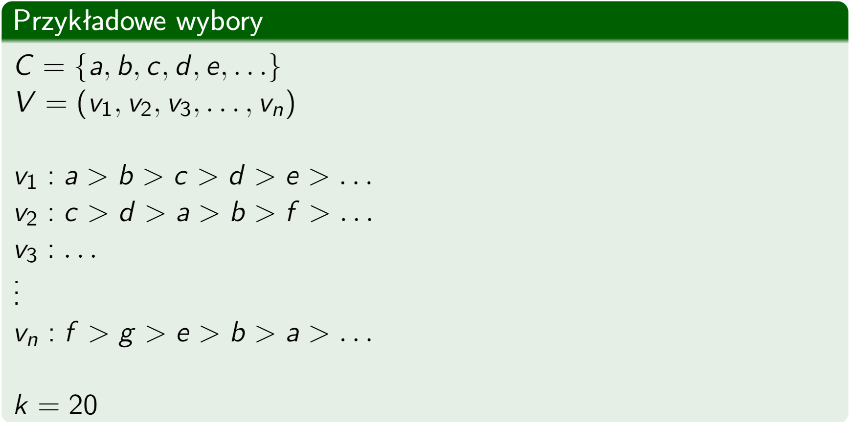
\includegraphics[width=0.8\textwidth]{pics/przykladowe_wybory.png}
\end{center}
Ciąg kandydatów przyporządkowany danemu wyborcy traktowany jest jako głos w
wyborach. Każdemu kandydatowi w ciągu stanowiącym głos, przyporządkowane są punkty
według punktacji Bordy. Jeżeli przez $i$ zostanie oznaczona pozycja danego kandydata w
ciągu stanowiącym głos (jeżeli kandydat jest pierwszy w ciągu, wtedy $i = 1$, jeśli drugi, wtedy $i = 2$ itd.), to wartość punktowa przyporządkowana według metody Bordy w tym głosie dla tego kandydata wynosi $\beta(i) = m - i$ , gdzie $m$ to rozmiar zbioru $C$ (liczba wszystkich kandydatów). Zatem dla danego głosu kolejni uporządkowani kandydaci otrzymują kolejno $m - 1, m - 2, … , 1, 0$ punktów.

\begin{center}

\includegraphics[width=0.8\textwidth]{pics/Borda_points.png}
\end{center}
W celu wyłonienia zwycięzców wyborów komitetów definiuje się tzw. funkcję satysfakcji,
która bazuje między innymi na punktacji metodą Bordy. Funkcja satysfakcji określa
zadowolenie danego wyborcy ze zwycięskiego komitetu. W celu zwięzłego zdefiniowania
funkcji celu wprowadza się pojęcie ciągu pozycji, które określa dla danego wyborcy pozycje
wszystkich zwycięskich kandydatów z jego preferencji. Ciąg pozycji jest posortowany
rosnąco - pozycja najbardziej preferowanego kandydata spośród zwycięzców na początku
ciągu, pozycja najmniej preferowanego kandydata spośród zwycięzców na końcu ciągu. \\  \\
Przykład \\ 
Dla następujących preferencji:

\begin{center}

\includegraphics[width=0.8\textwidth]{pics/positions.png}
\end{center}
komitetu $K = \left\{a, b, e\right\}$ i wyborcy $v_3$ ciąg pozycji oznaczany ${pos_v}_3$ wynosi $(3,4,6)$, gdyż pozycja najlepszego kandydata ze zbioru $K$ wynosi $3$ (kandydat $e$), druga najlepsza to pozycja nr $4$ (kandydat $b$), a ostatnią pozycją najmniej preferowanego kandydata jest pozycja nr $6$ (kandydat $a$). \\ \\
W tym momencie można zdefiniować funkcję satysfakcji, która jako argument przyjmuje
zdefiniowany przed chwilą ciąg pozycji, który dla każdego wyborcy $i$ dla każdego komitetu
jest określony jednoznacznie. Funkcja satysfakcji określająca zadowolenie danego wyborcy
ze zwycięskiego komitetu, będzie więc oznaczana jako $f(i_1, i_2, ... , i_k)$. \\ \\
Poprzez różne zdefiniowanie funkcji satysfakcji, definiowane są odmienne systemy
wyborcze. Znanymi systemami wyborczymi są system $k-Borda$ oraz system
$Chamberlin-Courant’a$. Funkcje satysfakcji dla tych systemów określone są odpowiednio:
$$f_{k-Borda}(i_1, i_2, ..., i_k) = \beta(i_1) + \beta(i_2) + ... + \beta(i_k) 
$$ $$f_{CC}(i_1, i_2, ..., i_k) = \beta(i_1) = max(\beta(i_1), \beta(i_2), ..., \beta(i_k))$$
Wyniki wyborów dla podanych systemów mogą być różne (i zazwyczaj są) pomimo takich
samych danych wejściowych. Inaczej rzecz ujmując, zwycięskie komitety mogą składać się z
różnych kandydatów po zastosowaniu odmiennych funkcji satysfakcji. \\ \\
Funkcja satysfakcji, która dotyczy niniejszego projektu inżynierskiego jest oparta na normie
$\ell_p$ . Norma $\ell_p$ zdefiniowana jest następująco:
$$\ell_p(x_1,x_2,\dots, x_n) = \sqrt[p]{x_1^p+x_2^p+\dots+x_n^p}$$
, gdzie $x_1, x_2, ..., x_n \in \mathbb{R}, p \in \mathbb{N}$ \\ \\
Dla skrajnych przypadków, gdy $p = 1$ i gdy $p \to \infty$ norma $\ell_p$ przyjmuje odpowiednio postać sumy: $$l_1(x_1, x_2,\dots, x_n) = x_1 + x_2 +\dots+ x_n$$ oraz postać operatora maksimum: $$l_\infty(x_1, x_2,\dots, x_n) = max(x_1, x_2,\dots, x_n)$$
\\ Mając zdefiniowaną normę $\ell_p$ można określić funkcję satysfakcji będącą tematem pracy. $$f_{{\ell_p}-Borda}(i_1, i_2, ..., i_k) = \ell_p(\beta(i_1), \beta(i_2), ..., \beta(i_k)) = \sqrt[p]{[\beta(i_1)]^p+[\beta(i_2)]^p+\dots+[\beta(i_k)]^p}$$
Funkcja jest uogólnieniem systemu $k-Borda$. Jeżeli za $p$ przyjęta zostanie wartość $1$,
zdefiniowana funkcja przyjmuje postać funkcji satysfakcji dla zwykłego systemu $k-Borda$. Dla $p$ dążącego do nieskończoności funkcja przyjmuje postać funkcji satysfakcji dla systemu
$Chamberlin-Courant’a$.

% ------------------------------------------------------------------------------------------

\subsection{Możliwości}
Obliczanie wyników wyborów dla systemu $\ell_p-Borda$ metodą typu brute-force jest
czasochłonne. Już dla stosunkowo niewielkich rozmiarem danych, algorytm jest nieużyteczny. Dlatego głównym zadaniem projektu jest zaprojektowanie i implementacja algorytmów heurystycznych, które możliwie dokładnie i możliwie szybko obliczają wyniki wyborów. Ponadto do zadań zespołu należy próba oceny działania stworzonych algorytmów heurystycznych.
\subsection{Motywacja do stworzenia projektu}
Jednym z głównym celów realizacji projektu jest chęć poznania różnych sposobów tworzenia
algorytmów heurystycznych oraz zastosowanie ich do rozwiązania problemów w
interesującej zespół tematyce, jaką jest sposób wyłaniania zwycięzców w wyborach i
związek między tym sposobem a satysfakcją wyborców ze zwycięzców. Ponadto zespół
chciał porównać pod różnymi względami różne algorytmy heurystyczne. Interesujące jest
zestawienie algorytmów pod względem dokładności obliczanych rozwiązań, czasu działania,
czy trudności w projektowaniu i implementacji. 

Drugą, istotną motywacją do stworzenia systemu jest możliwość wykorzystania go do wielu
bardzo różnych sytuacji. Zdefiniowanie wyborów, których wyniki ma liczyć system, może
dotyczyć różnego rodzaju wyborów. Mogą to być wybory ludzi do wszelakiego typu organów
władz na różnych szczeblach organizacji państwowych lub organizacji prywatnych. Wybory
nie muszą dotyczyć ludzi, a mogą polegać na selekcji innych rzeczy. Można zdefiniować
wybory na filmy, które zostaną odtworzone w trakcie podróży samolotem, czy podczas
seansu z rodziną i znajomymi. Mogą to być wybory na miejsca wspólnego wypadu znajomych na weekend. Wszędzie, gdzie ma sens zastosowanie preferencji (ułożenie
rzeczy od najbardziej do najmniej pożądanej) można wykorzystać stworzony system.
Dzięki stworzonemu systemowi według określonych wymagań, możliwe jest nie tylko
szybkie obliczenie wyborów na bazie wprowadzonych do systemu preferencji. Możliwe jest
sterowaniem sposobem obliczania wyborów według pożądanej reprezentatywności
zwycięskich kandydatów. Można decydować czy zwycięzcy wyborów będą tacy, że każdy
znajdzie wśród nich takiego, którego bardzo lubi, ale też taki, którego bardzo nie lubi. Czy
może zwycięzcy mają być tacy, że większość wyborców co prawda nie znajdzie wśród nich
bardzo pożądanego kandydata, ale jednocześnie nie znajdzie takiego, którego bardzo nie
lubi. Możliwy jest również wybór pośredni między wskazanymi dwoma rozwiązaniami.
Przykładowo, jeżeli użytkownik chce wybrać kilka filmów do wspólnego seansu z
przyjaciółmi i rodziną, to może zdecydować między różnymi opcjami. Jedną z opcji jest taki
wybór, aby wśród wybranych filmów każdy ze znajomych znalazł film, który mu bardzo
odpowiada, lecz jednocześnie znalazły się takie, które większości znajomych wyraźnie nie
odpowiadają. Druga możliwość to taka, w której wybrane zostaną filmy, które większości
znajomych ani za bardzo nie odpowiadają, ani za bardzo nie przeszkadzają. Pozostałymi
możliwościami są opcje pośrednie między wskazanymi.

\subsection{Użytkownicy}
Potencjalnymi użytkownikami systemu mogą być osoby i organizacje, które potrzebują
systemu wybierania kilku elementów spośród puli wszystkich elementów w taki sposób, aby
usatysfakcjonować swoich klientów. System może mieć przykładowe zastosowanie dla
przedsiębiorstw realizujących usługi transportu lotniczego czy autokarowego do umilenia
czasu podróży poprzez wybór odpowiednich filmów czy potraw. Ponadto system może
służyć pojedynczym osobom w celu wyboru odpowiedniej formy spędzania wolnego czasu w
grupie znajomych.

\subsection{Usługi dostarczanie przez system}

\subsubsection{Usługi wymagane}
\begin{itemize}
    \item możliwość wprowadzenia wyborów do systemu
    \item obliczenie wyników wyborów
    \item wyświetlanie wyników wyborów
\end{itemize}

\subsubsection{Usługi pożądane}
\begin{itemize}
    \item możliwość zarządzania swoimi wyborami (dodawanie nowych wyborów, nowych wyników, porównywanie różnych rezultatów)
    \item intuicyjna nawigacja po systemie
\end{itemize}

\subsubsection{Usługi dodatkowe}
\begin{itemize}
    \item wygodny sposób definiowania wyborów - zadanie projektowe koncentruje się na
projektowaniu i tworzeniu algorytmów obliczających wyniki wyborów. System musi
wczytywać pewien format pliku wejściowego definiującego wybory, który niekoniecznie jest prosty i intuicyjny w tworzeniu. Jeżeli ta dodatkowa usługa zostałaby zrealizowana, ułatwiłaby użytkowanie systemu i poprawiła zadowolenie użytkowników z korzystania z systemu
\end{itemize}

%-------------------------------------------------------------------------------------------
%-------------------------------------------------------------------------------------------
\section{Studium wykonalności}
  
\subsection{Opis wymagań}




% o ile to mozliwe prosze uzywac odwolan \cite w konkretnych miejscach a nie \nocite

%\nocite{artykul2011,ksiazka2011,narzedzie2011,projekt2011}

\bibliography{bibliografia}

\end{document}
